% !Mode:: "TeX:UTF-8"
%hithesis-alpha 用来测试添加开题/中期报告功能,非正式
%\documentclass[newtxmath=true,newgeometry=two,capcenterlast=true,subcapcenterlast=true,openright=true,absupper=true,fontset=windowsnew,type=doctor]{hithesis}
%\newcommand{\customheader}{testtest}
\documentclass[newtxmath=true,newgeometry=two,capcenterlast=true,subcapcenterlast=true,openright=false,absupper=true,noheader=false,stage=kaiti,type=master,tocfour=true]{hithesis}

%%开题去掉右翻页设置,openright=right改为false,大论文需改回来 _t
% 此处选项中不要有空格
%%%%%%%%%%%%%%%%%%%%%%%%%%%%%%%%%%%%%%%%%%%%%%%%%%%%%%%%%%%%%%%%%%%%%%%%%%%%%%%%
% 必填选项
% type=doctor|master|bachelor
%%%%%%%%%%%%%%%%%%%%%%%%%%%%%%%%%%%%%%%%%%%%%%%%%%%%%%%%%%%%%%%%%%%%%%%%%%%%%%%%
% 选填选项(选填选项的缺省值已经尽可能满足了大多数需求,除非明确知道自己有什么
% 需求)
% glue=true|false
% 	含义:由于我工规范中要求字体行距在一个闭区间内,这个选项为true表示tex自
% 	动选择,为false表示区间内一个最接近版心要求行数的要求的默认值,缺省值为
% 	false。
% tocfour=true|false
% 	含义:是否添加第四级目录,只对本科文科个别要求四级目录有效,缺省值为
% 	false
% fontset=siyuan|windowsnew|windowsold
% 	含义:注意这个选项视为了解决特殊问题而设置,比如用有些发行版本的linux排
% 	版时可能(大多数发行版不会)会遇到的字体无法载入的问题,或者字体载入之
% 	后出现无法复制的问题以及想要解决排版如 biang biang 面的 biang 这类中易
% 	宋体无法识别的汉字的问题。没有特殊的需要不推荐使用这个选项。
%
% 	如果是安装了 windowns 字体的 linux 系统,可以填写windowsnew(win vista
% 	以后 的字体)或 windowsold(vista 以前)或者想用思源宋体并且是已经安装
% 	了思源宋体的任何系统,填写siyuan选项。缺省值为空,自动识别系统并匹配字体
% 	。模板版中给出的思源字体定义文件定义的思源字体的版本是Adobe版,其他字体
% 	是windowsnew字体。
% tocblank=true|false
% 	含义:目录中第一章之前,是否加一行空白。缺省值为true。
% chapterhang=true|false
% 	含义:目录的章标题是否悬挂居中,规范中要求章标题少于15字,所以这个选项
% 	有无没什么用,除了特殊需求。缺省值为true。
% fulltime=true|false
% 	含义:是否全日制,缺省值为true。非全日制如同等学力等,要在cover中设置类
% 	型,封面中不同格式
% subtitle=true|false
% 	含义:论文题目是否含有副标题,缺省值为false,如果有要在cover中设置副标
% 	题内容,封面中显示。
% newgeometry=one|two
% 	含义:规范中的自相矛盾之处,版芯是否包含页眉页脚,旧方法是按照包含页眉
% 	页脚来设置。该选项是多选选项,如果没有这个选项,缺省值是旧模板的版芯设
% 	置方法,如果设置该选项one或two,分别对应两种页眉页码对应版芯线的相对位
% 	置。第一种是严格按照规范要求,难看。第二种微调了页眉页码位置,好一点。
% debug=true|false
% 	含义:是否显示版芯框和行号,用来调试。默认否。
% openright=true|false
% 	含义:博士论文是否要求章节首页必须在奇数页,此选项不在规范要求中,按个
% 	人喜好自行决定。 默认否。注意,窝工的默认情况是打印版博士论文要求右翻页
% 	,电子版要求非右翻页且无空白页。如果想DIY(或身不由己DIY)在什么地方右
% 	翻页,将这个选项设置为false,然后在目标位置添加`\cleardoublepage`命令即
% 	可。
% capcenterlast=true|false
% 	含义:图题、表题最后一行是否居中对齐(我工规范要求居中,但不要求居中对
% 	齐),此选项不在规范要求中,按个人喜好自行决定。默认否。
% subcapcenterlast=true|false
% 	含义:子图图题最后一行是否居中对齐(我工规范要求居中,但不要求居中对齐
% 	),此选项不在规范要求中,按个人喜好自行决定。默认否。
% absupper=true|false
%       含义:中文目录中的英文索引在中文目录中的大小写样式歧义,在规范中要求首
%       字母大写,在work样例中是全大写。该选项控制是否全大写。默认否。
% bsmainpagenumberline=true|false
%       含义:由于本科生论文官方模板的页码和页眉格式混乱,提供这个选项自定义设
%       置是否在正文中显示页码横线,默认否。
% bsfrontpagenumberline=true|false
%       含义:由于本科生论文官方模板的页码和页眉格式混乱,提供这个选项自定义设
%       置是否在前文中显示页码横线,默认否。
% bsheadrule=true|false
%       含义:由于本科生论文官方模板的页码和页眉格式混乱,提供这个选项自定义设
%       置是否显示页眉横线,默认显示。
% splitbibitem=true|false
%       含义:参考文献每一个条目内能不能断页,应广大刀客要求添加。默认否。
% newtxmath=true|false
%       含义:数学字体是否使用新罗马。默认是。
%%开题/中期报告需修改:
%		首先依然正常选择type=doctor/master/bachelor
%stage=kaiti,zhongqi
%		含义:开题报告或中期报告时选填,需放在type项前,去掉该项缺省为false本硕博毕业论文格式。
%noheader=true,
%		含义:全局“没有页眉”选项,某些老师可能要求开题、中期报告没有页眉,去掉该项缺省为false,页眉正常显示,如果在bachelor下使用,优先级高于bsheadrule。
%%%%%%%%%%%%%%%%%%%%%%%%%%%%%%%%%%%%%%%%%%%%%%%%%%%%%%%%%%%%%%%%%%%%%%%%%%%%%%%%
\fancyhf{}
\usepackage{hithesis}
\usepackage{amssymb}
\usepackage{graphicx}
\usepackage{booktabs}
\usepackage{threeparttable}
\usepackage{multirow}
\usepackage{algorithm} %format of the algorithm 
\usepackage{algorithmic} %format of the algorithm 
\usepackage{amsmath} 
\usepackage{xcolor}
\graphicspath{{figures/}}

\renewcommand{\algorithmicrequire}{\textbf{Input:}} 
\renewcommand{\algorithmicensure}{\textbf{Output:}}

%在下面添加自定义宏包、命令

%------------以下是自定义添加的宏包(下面为示例,可删除)------------------
\usepackage{leftidx} %左上标
\usepackage{multirow} %表格多行合并
\usepackage{slashed}	% 场论slash
\usepackage{cancel}

\usepackage{setspace} %用于调整多行公式间距, \begin{spacing}{1.6} \begin{equation}..\end{equation}\end{spacing}  !!!caution:使用宏包同时也会改变表格的行距需在每个表格\begin{table}后添加:\renewcommand\arraystretch{1.55}






%------------以下是自定义添加的命令(下面为示例,可删除)------------------

%重新定义section和subsection标号格式,去掉Chapter继承标号,因为开题等报告没有Chapter层级
%\renewcommand\thesection{\arabic {section}.}
%\renewcommand\thesubsection{\thesection \arabic {subsection}}

%-------罗马数字定义-------
\makeatletter
\newcommand{\rmnum}[1]{\romannumeral #1}
\newcommand{\Rmnum}[1]{\expandafter\@slowromancap\romannumeral #1@}
\makeatother


%---------正体字母定义------------
\newcommand{\ud}{\mathrm{d}}
\newcommand{\ue}{\mathrm{e}}
\newcommand{\ui}{\mathrm{i}}

%---------度°符号定义-------------
\def\degree{\ensuremath{{}^{\circ}}} 

%---------tabular行距------------
%\renewcommand{\arraystretch}{1.25}

	%插入自定义宏包、命令文件_t

\begin{document}

\frontmatter
%\setcounter{page}{0} %如果使用开题/中期报告时,目录页码不正确时使用,重置页码计数器
%\includepdfmerge{front/report_cover.pdf}	
%如果自动生成封面不满足需要,可以自行填写学校word模板封面,生成pdf文件,放入front文件夹,手动插入该pdf封面,并手动注释掉下面% !Mode:: "TeX:UTF-8"
%开题/中期报告封面页
\hitsetup{
  %******************************
  % 注意:
  %   1. 配置里面不要出现空行
  %   2. 不需要的配置信息可以删除
  %******************************
  %
  %=====
  % 秘级
  %=====
  %
  %=========
  % 中文信息
  %=========
  ctitleone={时间序列数据}, %论文题目,第一行此处最多12个字,多出的字放在\ctitletwo
  ctitletwo={异常检测关键技术研究}, %论文题目第二行,第一行放不下的文字,放在这里
  csubject={计算机科学与技术},
  caffil={机电工程学院},
  cauthor={靳贺霖},
  csupervisor={王宏志教授},
  ccosupervisor={某某某教授}, % 联合指导老师
  % 日期自动使用当前时间,若需指定按如下方式修改:
  cdate={2020/3/25},
  cstudentid={1160300312},
  %cstudenttype={同等学力人员}, %非全日制教育申请学位者
  %(同等学力人员)、(工程硕士)、(工商管理硕士)、
  %(高级管理人员工商管理硕士)、(公共管理硕士)、(中职教师)、(高校教师)等
  %
  %
  %配置
  %\renewcommand\thesection{\arabic {section}.}
  %\renewcommand\thesubsection{\thesection \arabic {subsection}}
  %\setcounter{page}{0}
}  及 \makecover 两行。
% !Mode:: "TeX:UTF-8"
%开题/中期报告封面页
\hitsetup{
  %******************************
  % 注意:
  %   1. 配置里面不要出现空行
  %   2. 不需要的配置信息可以删除
  %******************************
  %
  %=====
  % 秘级
  %=====
  %
  %=========
  % 中文信息
  %=========
  ctitleone={时间序列数据}, %论文题目,第一行此处最多12个字,多出的字放在\ctitletwo
  ctitletwo={异常检测关键技术研究}, %论文题目第二行,第一行放不下的文字,放在这里
  csubject={计算机科学与技术},
  caffil={机电工程学院},
  cauthor={靳贺霖},
  csupervisor={王宏志教授},
  ccosupervisor={某某某教授}, % 联合指导老师
  % 日期自动使用当前时间,若需指定按如下方式修改:
  cdate={2020/3/25},
  cstudentid={1160300312},
  %cstudenttype={同等学力人员}, %非全日制教育申请学位者
  %(同等学力人员)、(工程硕士)、(工商管理硕士)、
  %(高级管理人员工商管理硕士)、(公共管理硕士)、(中职教师)、(高校教师)等
  %
  %
  %配置
  %\renewcommand\thesection{\arabic {section}.}
  %\renewcommand\thesubsection{\thesection \arabic {subsection}}
  %\setcounter{page}{0}
} % 开题/中期封面
%% !Mode:: "TeX:UTF-8"

\hitsetup{
  %******************************
  % 注意:
  %   1. 配置里面不要出现空行
  %   2. 不需要的配置信息可以删除
  %******************************
  %
  %=====
  % 秘级
  %=====
  statesecrets={公开},
  natclassifiedindex={TM301.2},
  intclassifiedindex={62-5},
  %
  %=========
  % 中文信息
  %=========
  ctitleone={局部多孔质气体静压},%本科生封面使用
  ctitletwo={轴承关键技术的研究},%本科生封面使用
  ctitlecover={局部多孔质气体静压轴承关键技术的研究},%放在封面中使用,自由断行
  ctitle={局部多孔质气体静压轴承关键技术的研究},%放在原创性声明中使用
  csubtitle={一条副标题}, %一般情况没有,可以注释掉
  cxueke={工学},
  csubject={机械制造及其自动化},
  caffil={机电工程学院},
  cauthor={于冬梅},
  csupervisor={某某某教授},
  cassosupervisor={某某某教授}, % 副指导老师
  ccosupervisor={某某某教授}, % 联合指导老师
  % 日期自动使用当前时间,若需指定按如下方式修改:
  %cdate={超新星纪元},
  cstudentid={9527},
  cstudenttype={同等学力人员}, %非全日制教育申请学位者
  %(同等学力人员)、(工程硕士)、(工商管理硕士)、
  %(高级管理人员工商管理硕士)、(公共管理硕士)、(中职教师)、(高校教师)等
  %
  %
  %=========
  % 英文信息
  %=========
  etitle={Research on key technologies of partial porous externally pressurized gas bearing},
  esubtitle={This is the sub title},
  exueke={Engineering},
  esubject={Computer Science and Technology},
  eaffil={\emultiline[t]{School of Mechatronics Engineering \\ Mechatronics Engineering}},
  eauthor={Yu Dongmei},
  esupervisor={Professor XXX},
  eassosupervisor={XXX},
  % 日期自动生成,若需指定按如下方式修改:
  edate={December, 2017},
  estudenttype={Master of Art},
  %
  % 关键词用“英文逗号”分割
  ckeywords={\TeX, \LaTeX, CJK, 嗨!, thesis},
  ekeywords={\TeX, \LaTeX, CJK, template, thesis},
}

\begin{cabstract}

摘要的字数(以汉字计),硕士学位论文一般为500 $\sim$ 1000字,博士学位论文为1000 $\sim$ 2000字,
均以能将规定内容阐述清楚为原则,文字要精练,段落衔接要流畅。摘要页不需写出论文题目。
英文摘要与中文摘要的内容应完全一致,在语法、用词上应准确无误,语言简练通顺。
留学生的英文版博士学位论文中应有不少于3000字的“详细中文摘要”。

  关键词是为了文献标引工作、用以表示全文主要内容信息的单词或术语。关键词不超过 5
  个,每个关键词中间用分号分隔。(模板作者注:关键词分隔符不用考虑,模板会自动处
  理。英文关键词同理。)
\end{cabstract}

\begin{eabstract}
   An abstract of a dissertation is a summary and extraction of research work
   and contributions. Included in an abstract should be description of research
   topic and research objective, brief introduction to methodology and research
   process, and summarization of conclusion and contributions of the
   research. An abstract should be characterized by independence and clarity and
   carry identical information with the dissertation. It should be such that the
   general idea and major contributions of the dissertation are conveyed without
   reading the dissertation.

   An abstract should be concise and to the point. It is a misunderstanding to
   make an abstract an outline of the dissertation and words ``the first
   chapter'', ``the second chapter'' and the like should be avoided in the
   abstract.

   Key words are terms used in a dissertation for indexing, reflecting core
   information of the dissertation. An abstract may contain a maximum of 5 key
   words, with semi-colons used in between to separate one another.
\end{eabstract}
 % 毕业论文封面
\makecover
%\begin{denotation}
\begin{table}[h]%此处最好是h
\caption{国际单位制中具有专门名称的导出单位}
\vspace{0.5em}\centering\wuhao
\begin{tabular}{ccccc}
\toprule[1.5pt]
量的名称&单位名称&单位符号&其它表示实例\\
\midrule[1pt]
频率&赫[兹]&Hz&s-1\\
\bottomrule[1.5pt]
\end{tabular}
\end{table}
\end{denotation}
%物理量名称表,符合规范为主,有要求添加
%\cleardoublepage  %自定义在什么位置进行右翻页
\tableofcontents    % 中文目录,有些专业研究生开题要求添加目录,中期、本科不要求,以教学秘书发送模板要求为准, 自行添加
%\cleardoublepage  %自定义在什么位置进行右翻页
%\tableofengcontents % 英文目录,硕本不要求,开题/中期不要求

\mainmatter
%\linenumbers %debug 选项
%\layout %debug 选项
%\floatdiagram %debug 选项
%\begin{figure} %debug 选项
%\currentfloat %debug 选项
%\tryintextsep{\intextsep} %debug 选项
%\trytopfigrule{0.5pt} %debug 选项
%\trybotfigrule{1pt} %debug 选项
%\setlayoutscale{0.9} %debug 选项
%\floatdesign %debug 选项
%\caption{Float layout with rules}\label{fig:fludf} %debug 选项
%\end{figure} %debug 选项
\section{课题来源及研究的背景和意义}

\subsection{课题的来源}

项目来源:国家自然科学基金项目(编号:U1509216,U1866602)

\subsection{课题研究的背景和意义}

随着各种新兴产业的发展,包括各种应用领域,如医学,生物学,以及交通领域等,我们能从各种装置上收集得到大量的带有时间戳的多维数据,有效地分析这些时间序列数据能够帮助相关产业更好地将数据转换成效益。但是在这些大量的数据中,一些数据会表现出不正常的行为或者模式。事实上,这些异常点(Outliers)可能是由于噪声造成的,这时候我们要将其修复或者去除;或者它们表示着我们比较感兴趣的一些事件,如机器故障,恐怖袭击等。根据不同的目的要展开不同的分析\cite{koufakou2010fast}。

事实上,在数据分析领域,发现异常点一直都是比较受欢迎的一个研究方向,因为它能够找出数据中的不正常的行为。而且,现在在数据分析的过程,异常检测并处理已经成为一个十分必要的预处理过程\cite{ha2014robust}。比如,在机器学习领域,数据质量对模型表现的影响是非常大的,噪声数据可能会阻碍模型挖掘出需要的信息,所以在执行数据预处理过程中常常把异常检测作为比较重要的一环\cite{zhang2017time}。

异常检测(Outlier Detection)也是一个挖掘信息的过程。除了是数据噪声造成的异常外,异常数据往往还代表着不正常事件的发生。许多领域都对应用异常检测方法来挖掘特殊信息感兴趣,比如说恐怖袭击检测\cite{riffo2015automated}、欺诈发现、健康管理和故障调试与诊断\cite{allen2011anomaly}等。这些领域研究都有一个共同的特征,即需要检测到的行为是和正常行为是不同的,这和异常检测的定义相吻合。

时间序列(Time Series)数据不仅有着现如今数据高维,量大\cite{budalakoti2006anomaly}的特点,还有着时序特征。传统的一些数据异常检测方法在时间序列数据上是可以使用的,但是由于没有考虑数据的时序特征往往得到的结果并不理想。而且,时序数据常常表现出强烈的短期依赖性(Temporal Dependence)\cite{cai2018effective},这就对时间序列异常检测有了更高的要求。虽然现在已经有很多关于时间序列异常检测的方法,但是仍然很难满足对现如今数据发展的要求。

\section{国内外在该方向的研究现状及分析}

已有的时间序列异常检测的方法可以分为不同的类别,不同的类别有着不同的优势和劣势。接下来几个章节主要来讲国内外已有的一些方法,并主要分析他们的优势和劣势所在。

\subsection{基于概率统计模型的时间序列数据异常检测}

基于统计的异常检测方法主要是通过数据的一些统计特征来进行异常检测的,比如说一个数据库中的数据是大致符合某个统计模型,那么异常数据往往对这个统计模型不适用或者出现的概率很低\cite{eskin2000anomaly,hido2011statistical}。但是,一方面这些方法不能够很好地移植到时间序列数据异常检测中;另一方面,随着数据维度的不断增多,传统的统计模型已经无法适应异常检测的要求。不过虽说如此,仍然有一些比较好的能够处理时间序列数据的统计模型。

Zhang et al.\cite{zhang2016sequential}应用了前人使用的基于对时间序列数据值变化速度约束从而进行异常检测的方法\cite{song2015screen}。但是传统的方法有一个缺陷是虽然它能够很好地检测出大幅度变化的异常,但是却很难检测出较小变化的异常。为此,作者改善了原文献中的依靠变化速度的最大最小值约束来进行异常检测,而是通过对速度的变化进行概率建模,并最大化似然来估计异常。巧妙地使用了概率模型来提高了异常检测的精度。

Guo et al.\cite{guo2010improved}通过分段聚集估计方法先对时间序列数据分段,随后在段上定义了几种统计特征值。然后定义了几种衡量分段聚集估计方法段之间距离方法,这些方法是通过前面计算的统计特征值来实现的。通过这些距离的定义可以计算段之间的差异程度,亦可以通过定义的距离来对时间序列数据进行异常检测。

其实,早先基于概率统计模型的时间序列异常检测的方法较多。但是这些模型大都已经不能够适应现在时间序列数据的要求,数据量越来越大,数据维度越来越高,逐渐就淘汰掉了这些方法。但是它们有着处理效率高,速度快的特点,作为预处理的一环也不失为一种好方法。

\subsection{基于机器学习的时间序列数据异常检测}

机器学习运用到时间序列数据管理已经有了很多方面的研究\cite{laure2018machine},异常检测方法有很多是基于机器学习方法来实现的,根据机器学习方法分类可以分为监督学习和无监督学习,这主要是由数据是否有标签来决定的\cite{chandola2009anomaly}。

在有标签的训练数据上,就可以使用监督学习的方法。常常在异常检测方面,会将异常检测问题转换为一个二分类问题\cite{gupta2013outlier}。在数据集标签存在的情况下,传统的二分类算法都能够应用到异常检测上。如使用传统的监督学习算法,决策树、朴素贝叶斯、SVM的基于特征分来的算法来进行对时间序列数据进行异常检测的\cite{kang2005learning},也有使用滑动窗口进行取数据段,然后通过对数据段进行提取特征,使用SVM进行分类的方法\cite{tian2007sequence,wang2006native}。还有对数据进行采样进行多次分类算法的,如这篇文献\cite{gonzalez2003anomaly}中,作者选择使用否定选择算法,而不是其他算法常用的抽样阳性(正确的)数据。通过将对正常数据和异常数据进行采样,使用分类算法,得到异常数据的特征并以此进行异常检测。

监督学习的方法在数据存在标签的时候是可以有比较不错的表现的,而且使用时间序列的子串来进行分类也有着不错的结果\cite{le2017time}。但是关于监督学习的方法大都是十年前的研究,因为有标签的数据集比较难得。尤其是在现在数据量不断增大,数据维度不断增多的情况。传统的标签方法常常是人工经验备注,但是数据量变大以后这种方法就变得不太现实。所以监督学习应用于时间序列数据的异常检测往往不多。

聚类是比较有代表性的无监督方法,传统的聚类方法实现的关键主要是距离的衡量,根据不同的时间序列数据库来挑选距离衡量方法是很重要的一个过程\cite{mori2015similarity}。距离衡量的方法确定后就是聚类方法的选择,传统的\(k\)-Means,GMM等都是可以使用的。异常检测过程主要就是判断数据点到它所属中心的距离来当作它的异常打分。但是,传统的聚类方法在时间序列上表现一般,除此还有使用基于托普利兹矩阵以及马尔科夫随机场(Toeplitz Inverse Covariance-based Clustering)来对时间序列数据自序列进行聚类的方法\cite{hallac2017toeplitz},很好的解决了传统聚类方法丢失时序特征的问题。

无监督方法除了聚类,还有使用主成分分析(Principal Component Analysis, PCA)来对时间序列数据进行预测和异常检测的\cite{papadimitriou2005streaming}。这篇文章的思路大概是通过主成分分析最小化重构误差来获得时间序列数据的隐空间,然后增量训练,数据点可以带入到训练好的模型中计算输入和输出的距离来当作异常打分,从而实现异常检测。而且,为了强调时间序列数据的短期依赖性,增量训练模型的过程会给以往的模型添加遗忘因子减少权重。

还有一种构造模型的方法和聚类有点类似\cite{chan2005modeling}。对于时间序列数据,它会构建出一些box,这种方法类似于聚类中常使用的自底向上的层次聚类方法。不同的是这种方法只考虑时间序列数据中相邻数据的结合。在训练过程中,首先每个数据独立当作一个box,计算相邻box的距离并将最小的那两个合并,其中距离的计算用两个box之间点距离的最小值来得到。然后重复这个操作直到得到了k个box(k为需要指定的参数)。在测试过程中,如果新到来的数据在当前的box中,那么它的异常得分(anomaly)为0,否则就计算它和最近的box的距离,并和设置的阈值进行对比,如果超出阈值的话就说明这个点是一个异常点。

还有一种增量建立模型的方法是通过支持向量回归机(Support Vactor Regerssion, SVR)来实现的\cite{ma2003online}。SVR和SVM类似,只是SVR要寻找的最优超平面是使所有的样本点离着超平面的总偏差最小。作者建立了一个异常检验的模型,包括预测模型,异常区间,异常数量等等,然后将SVR代入到这个模型中。当前时刻预测下一个点的值(离超平面近的点)然后与实际的值进行对比,通过异常区间的阈值来判断该点是否异常,并将这个点加入到模型中重新构造模型。

除了这些方法外,其实还有很多无监督方法能应用于时序数据异常检测,如隐马尔科夫模型(Hidden Markov Models, HMMS)\cite{florez2005efficient},有穷状态机(Finite state Automata, FSA)\cite{chandola2008comparative}等等。

基于距离的时间序列研究方法可行的原因是十分直观的:一个观测点如果距离离他最近的点都很远的话,那么它就很有可能是一个异常点。做法也比较直观,首先找到所有点距离它最近的点,然后以最近点的距离当作权值对所有的所有点排序,那些距离大的点就可以被当作是异常点,这是比较经典的一篇实现\cite{huang2013rank}。

所以,对这种方法而言,距离的定义就成为比较重要的一环。在定义距离的这些方法中,$k$NN是经常使用的一种方法。一种方法是以$k$NN中$k$个点的最远距离当作距离的衡量\cite{ramaswamy2000efficient},另一种方法是以$k$NN中$k$个点的距离和当作距离的衡量\cite{angiulli2002fast}。除此,为了加速对$k$NN的查询,还有在数据集上建立最小生成树,从而加快对$k$NN的查询来实现异常检测的\cite{wang2015fast}。

基于距离的时间序列数据异常检测有很大的优点,即算法简单高效。而且,如果以时间序列数据的数据段为单位进行距离衡量的话往往能比较高效地查询到数据中存在的区间异常。但是也存在很大的缺陷,对时间序列数据的距离衡量来说,一方面,数据的维度很大,距离衡量在一方面会受某个维度的影响。而且,当数据量很大的时候,可能异常点的数量也会随之增大,造成使用$k$NN等的方法不能够很好地找到异常数据\cite{aggarwal2015outlier}。

\subsection{基于深度学习的时间序列数据异常检测}

基于深度学习的时间序列数据异常检测是近年比较热门的研究方向。尤其在卷积神经网络(Convolutional Neural Network, CNN)以及循环神经网络(Recurrent Neural Network, RNN)中表现比较突出。在时间序列上的应用大致分两个方面:一方面是通过神经网络来对时间序列数据进行预测,通过比较预测值和原始数据的距离来判断异常;另一方面是使用自编码器最小化重构误差\cite{srivastava2015unsupervised}来实现。

具体来说,有使用循环神经网络的变种长短期记忆模型(Long Short-Term Memory, LSTM)对时间序列数据进行预测并以此进行异常检测的方法\cite{filonov2016multivariate}。这种方法通过对数据进行分段,得到一个数据段序列,然后以数据段的顺序分别以相邻的两个数据段当作长短期记忆模型的输入和输出,异常检测通过计算预测值和实际值的MSE来打分实现。

也有使用多层卷积网络最小化重构误差训练模型并以此异常检测的方法\cite{kieu2018outlier}。通过多层的卷积网络,首先把原始数据降维,然后再升维,训练过程中使升维后的结果等于原始数据段,这样就能够得到包含数据信息的隐空间。异常检测过程就计算输入和输出的MSE当作异常打分。

除此,最近的工作中还有使用稀疏连接的循环神经网络(Sparsely-connected Recurrent Neural Networks, S-RNN)来生成多种自编码器,这些自编码器分为多种不同的结构,然后仍然通过最小化重构误差来训练模型,通过计算输入和输出的MSE来做当异常打分获得异常数据\cite{kieu2019outlier}。

此外,还有使用生成对抗网络来对时间序列数据进行异常检测的\cite{li2019mad}。作者通过训练生成对抗网络,形成产生器(generator)和判别器(discriminator),对抗网络内部通过LSTM-RNN实现,也在网络攻击数据上取得了不错的效果。

深度学习的方法在多维数据上表现很好,而且循环神经网络等也能很好地适应时间序列数据处理的要求,但是这些准确性都是基于复杂的神经网络和高密度的训练过程的。现如今随着数据量、数据维度的不断增大,训练神经网络让这个过程不太轻松。

\subsection{半监督学习以及基于半监督学习的异常检测}

\subsubsection{半监督学习研究进展}

机器学习领域中的半监督学习已经有了比较多的相关研究\cite{Hady2013Semi},这里就不对一些年代久远的方法进行赘述了。主要讨论一下近期半监督学习领域的研究进展以及半监督学习在异常检测技术上的一些利用。

Kingma et al.\cite{Kingma2014Semi}将无监督的变分自编码器扩展成为了两种不同形式的半监督模型。其中的M1是一种比较简单潜在特征判别模型,在样本的潜在表示顶端,训练出一个分类器来预测标签。在对变分自编码器的训练过程中,有标签和无标签数据都被使用了,但是分类器是使用有标签的数据来训练的。另一种M2则就相对复杂一些。除了在样本潜在表示顶端使用分类器外,还由另一个由标记数据和未标记数据共同生成的类别变量有关。最后,可以通过将M1模型的嵌入表示来学习M2来将M1和M2模型进行结合。除了这篇比较有代表性以外,\cite{siddharth2017learning, sonderby2016ladder}也是对自编码器进行扩展,从而形成半监督模型。

生成对抗网络GAN也主要通过两个方面来进行半监督学习。其中一种是考虑生成K+1个分类器,其中前K个用于对给定的标签数据进行分类,然后对于未标记数据,将其带入到训练好的前K个分类器中来得到他们的分布,然后使用特征匹配技术来解放竞争性性能\cite{DBLP:journals/corr/SalimansGZCRC16}。另一种考虑将学习的GAN模型的生成器作为流形学习的参数化,可以通过流形切线来表示数据的标签\cite{DBLP:conf/cvpr/QiZHEWH18}。

此外,teacher-student模型也是近些年来半监督学习研究的主要模型之一。其思想大致是首先通过有标签数据获得一组教师,然后使对无标签数据的预测作为学生,通过教师来监督学生的学习,通过最大化教师和学生之间的一致性,来提高学生对无标签数据进行分类时的准确性和稳定性。按照不同的强化教师和学生一致性的方法,可以将模型分为不同的种类。

比如说通过在模型的输入层和隐藏层添加噪声\cite{DBLP:journals/jmlr/SrivastavaHKSS14}来提高模型的性能。这个的思想其实和在目标函数中添加正则项是类似的。在teacher-student模型中,将添加了噪声的样本输入到模型中,从而能够获得一个有噪声的teacher,然后将预测偏差最小化,在teacher和student之间训练模型。这就是teacher-student模型中的Γ模型\cite{DBLP:conf/nips/RasmusBHVR15}。或者在两个损坏的副本之间训练,这就是teacher-student模型中的Π模型\cite{DBLP:conf/iclr/LaineA17}。

除此,这些想法还扩展到了在时间上训练一群教师,让他们来临时的指导学生来学习,然后通过使用他们的指数移动平均值来提高教师对无标签数据预测的准确性\cite{DBLP:conf/iclr/LaineA17}。亦或者通过对模型的参数进行指数加权平均,形成对集成化教师的预测,这种做法也被叫做Mean Teacher\cite{DBLP:conf/iclr/TarvainenV17}。这些方法都依赖于添加到输入样本和模型参数中的随机噪声,从而加强训练过程中教师和模型预测结果之间的一致性,以及对无标签数据预测标签的稳定性。

teacher-student模型还有另外一种优化方法,不是通过添加噪声来实现的,而是产生一个对抗性老师。通过使教师于对抗化示例的偏差最小化的思想来训练和更新学生。这样就产生了新的方法——虚拟对抗训练VAT\cite{DBLP:journals/pami/MiyatoMKI19}。这也是半监督学习领域目前有state-of-the-art标签的算法。

\subsubsection{基于半监督学习的异常检测研究}

使用半监督学习来进行异常检测一直是异常检测领域比较空缺的一部分。一方面,异常检测数据按标签的分布往往是不均衡的,这就导致分类算法直接使用于异常检测领域效果不好。另一方面,由于异常数据的随机性,往往无法得到所有情况下异常数据的分布,只靠给定的少部分异常数据很容易在训练过程中过分拟合这些数据。因此业界也常常使用无监督学习来进行异常检测。但是,无监督学习对数据分布进行的假设过强,在一些数据上就可能会存在瓶颈。而且在现实中我们是可以通过专家或者经验来获得一部分数据标签的\cite{DBLP:conf/cvpr/BilenV16}。合适地使用这些少量的标签是能够学习出更多的特征,达到比无监督学习更好地效果的。下面来介绍一下使用半监督学习来进行异常检测的一些研究。

前面我们提到使用自编码器来进行异常检测的方法。我们训练的过程是直接将所有的训练数据代入到自编码器中,然后使用自编码器来进行异常检测。这里我们是将训练数据中的未知标签的正常数据和异常数据都作为输入和输出训练出的自编码器。因为数据中异常数据很少,所以我们学习到的大部分都是正常数据的特征。\cite{DBLP:conf/mlsp/MunawarVM17}认为这种做法可能会使网络学习到异常数据的特征,从而降低了学习的准确性。因此他提出了一种半监督学习方法,通过改变代价函数,强制使正常数据最小化重构误差,异常数据最大化重构误差来强化对抗网络的重构能力。但是我觉得这种方法是存在一定的问题的。因为有标签数据的稀少,这样使少量的以上数据强制最大化重构误差会使模型过分拟合这部分异常数据,泛化能力较差。

另一种半监督学习异常检测算法使用了k-means的思想。通过在所有数据上(包括标签数据和无标签数据)进行聚类,然后在每一个簇上,通过整合其中所有有标签的数据的标签来判断这个簇的特征,从而判断这个簇上是否有异常数据\cite{DBLP:conf/sac/GaoCT06}。这是一种比较简单的方法。

还有一种半监督学习异常检测方法只使用正常数据和大量的无标签数据来进行异常检测\cite{DBLP:journals/ijait/DaneshpazhouhS15}。主要是思想是,首先通过$k$NN算法,来提取出一些比较可靠的异常数据。这部分主要是通过那些有标签的正常数据和所有数据的分布来实现的。然后对于获得的数据标签,使用Fuzzy Rough Semi-Supervised Outlier Detection\cite{DBLP:journals/mcs/XueSF10}算法来检测异常数据。这部分主要是通过一个概率矩阵来实现的。这个算法在异常检测方面优于无监督学习的最新技术。

直接使用半监督学习进行异常检测在部分情况下是优于无监督学习异常检测技术的。但是由于数据集中正常数据和异常数据不均衡是难以解决的问题,导致半监督学习分类算法在异常检测领域难以有好的结果。常常在训练过程中因为异常数据标签少而导致过分拟合异常数据,此时常常只能检测出一种或者几种异常。

\subsection{基于元学习的异常检测模型}

近两年也有元学习应用到异常检测领域的。Zhao et al.\cite{DBLP:journals/corr/abs-2009-10606}就使用元学习为不同场景下的数据挑选合适的无监督学习网络模型。他们提出的METAOD包含两个过程,首先是离线的元学习训练,通过计算不同模型在随机初始化的数据集上的性能表现,训练挑选出标签最好的网络模型,而且还引用了很多AutoML中常用的特征,包含最大值、最小值、均值、方差等。在线的检测就是通过训练得到的模型实时地提供性能最好的网络模型。这个网络模型其实更像是使用元学习来做网络模型的推荐,而不是之间使用元学习来进行异常检测。

Ding et al.\cite{DBLP:conf/www/DingZT021}在图异常检测领域使用了元学习。这篇论文面向的同样也是小样本学习的场景,提出了一种新的图偏差网络(GND)。它可以利用少量的标记异常来解决小样本学习网络检测过程中遇到的异常。同时为提出的GND提出了跨网络的元学习算法,通过从多个辅助网络传输元知识来实现小样本的异常检测。这部分研究就是直接在小样本学习网络中应用到了元学习,获得了不错的检测结果。

Tomoharu et al.\cite{DBLP:journals/corr/abs-2103-00684}使用one-class分类器进行异常检测,这种分类器既可以只使用正常数据来进行异常检测,也可以运用异常样本来提高算法的准确性。然后通过元学习的思路和特征提取的思路训练并迁移网络模型,最后训练得到最终的版本。这个研究跟我进行的度量学习有点像,也是将数据映射到嵌入空间后使用one-class分类器来进行异常检测,检测数据是否为正常样本,否则就为异常。

目前来说,元学习在时间序列异常检测方面的研究还是比较少,但是元学习的小样本学习能力可以适用到异常检测来,这也是我毕设想做的一部分内容之一。

\subsection{国内外文献综述的简析}

现在相对而言,时间序列异常检测已经有了许多可行的解决方案,分为不同的方面。这些研究成果在许多领域都有了应用而且产生了不错的效益。基于概率统计的模型在之前集群算力不够的时候是常用的方法,而且早先的数据并不像现在这样数据量大、数据维度高。但是现如今的数据呈现量大、维度高、关联性强等特点,一些简单的概率统计模型已经无法适应现在的要求。所以一些深度学习方法逐渐地也被应用到异常检测来。整体来讲,现在业界还存在一下几个问题:

\begin{itemize}
    \item 数据量和数据维度不断地增大,传统的机器学习等方法在适应高维度和大量数据上显得越来越吃力,处理需要的时间已经逐渐增加到无法接受的地步;
    \item 传统的异常检测算法不能达到时间序列异常检测的要求。因为时序特征是时间序列的重要特征,其明显特征就是短期依赖较强,如何合理的提取时间序列中的时序特征是亟待解决的问题;
    \item 真实场景下的标签数据难以获取,而一些领域的先验知识无法得到运用,所以如何融合大量的无标签数据和知识是一个很重要的问题;
    \item 小样本场景下的异常检测目前的研究较少。
\end{itemize}

我的毕设研究主要就是基于这几个问题来进行。

\section{主要研究内容}

我的毕业设计的研究内容主要从数据标签的获取难易程度入手,主要分为以下几点:

\begin{itemize}
    \item 无监督学习时间序列异常检测算法:无需数据标签就可以使用的异常检测算法,通常通过计算数据的离群程度来判断数据是否为异常点;
    \item 半监督学习时间序列异常检测算法:可以利用起有限标签的异常检测算法,因为真实的场景是我们常常可以获取到一部分先验知识,这些先验知识可以转换为部分数据的标签,利用起这部分标签能更有效地进行异常检测;
    \item 小样本学习时间序列异常检测算法:和半监督不同,这里着重研究的元学习、迁移学习等在时间序列异常检测领域的使用,在时间序列的场景下,如何利用已有的模型、知识,通过少量数据微调来获得更好的性能。
\end{itemize}

\subsection{不使用数据标签:无监督学习时间序列异常检测算法}

具有无监督学习算法是异常检测算法中使用频率最高的,现在很多研究和基准的异常检测算法都是基于无监督学习的。因为无监督学习模型在使用的时候不需要标注的数据,用起来简单,更适用于大多数场景,所以现在多数异常检测的研究方向都是在无监督学习上的。

自编码器是一种常见的神经网络模型,它可以用来做数据压缩、数据编码等,而且它天然的提取低维特征——重构原数据的模式使其能够用于异常检测领域。目前自编码器在异常检测领域已经有了一些研究,但是在时间序列的异常检测方面研究还是相对较少,而且现有的时间序列异常检测模型都相对简单,如PAA-AE,LSTM-AE和CNN-AE等。所以我考虑从这个方面入手,设计并实验验证得到一个真正适用于时间序列的异常检测自编码器模型。

考虑到现有的网络模型对时间序列的特征提取都不够:单独的RNN对时序数据的特征提取已经无法满足高维数据的要求,而非循环的神经网络又无法获得时序数据中的长期依赖,所以在未来的研究中,我想能够融合一些现在表现比较好的特征提取模型,包含时序特征的抽取和高维数据的抽取等。然后再根据这个模型构建一个自编码器用于异常检测,同时在实验验证中不断验证模型是否有更好的结果。

\subsection{使用部分标签:基于度量学习的时间序列异常检测算法}

无监督学习因为其适用性广、门槛低等优点被广泛应用,但是它的对应的归纳偏置却限制了它准确性:无监督学习异常检测算法是假定数据分布密集的部分是正常数据分布的范围,而离群点大多分布在偏离数据分布密集的位置。这种归纳偏置符合我们的直观认知,但是在一些场景下,它却也是不合理的。如风电机产生的数据中,异常包括Sparse Outliers和Stacked Outliers,其中的Stacked outliers就是聚集分布的异常点,使用传统的无监督异常检测方法会将这些数据误判为正常点。但是其实此时我们是知道这部分点的异常情况的,无监督学习方法无法利用这些知识帮助检测异常。

所以,如果能够利用起少量的数据标签用于辅助异常点的决策,如在前面的例子中,能否利用起已知的Stacked Outliers先验,告诉模型这部分堆积的数据也是异常数据呢?我们知道,监督学习是能够利用起数据中的标签的,但是,监督学习面向的是标签的数据,我们现在仅有部分标签和先验知识,如果只在这些数据上使用监督学习的话,又会使模型过拟合于这部分数据。所以,我们需要既利用起有限的标签和知识,也要利用起大量的无标签数据来辅助对异常点的判断,这其实就是半监督学习的思路。

想到半监督学习的异常检测,我们很容易就能想到使用半监督的分类模型来解决,将正常和异常的样本视为两类,转换为一个二分类问题。但是实际上,异常检测问题并不能简单地被归纳为二分类问题,因为通常情况下异常数据的特征是不可控的,即我们无法通过一种统一的模式来识别所有的异常。通常在异常检测领域的做法是,转换为单分类问题(one-class classification)。

基于这一点入手,我未来会从度量学习入手。原来的度量学习是针对分类问题,将数据映射到一个理想的嵌入空间上。嵌入的规则就是使相同类比的数据进行成簇分布。在异常检测方面,和分类问题会有很大的不同。暂定的想法是,使所有的正常样本在嵌入空间中尽量地聚簇分布,而使异常样本距离正常样本的距离尽量地远,通过神经网络将数据映射到这样的一个嵌入空间中,从而根据嵌入的数据到正常簇的距离,判断数据是否异常。这个过程需要适合的网络模型设计和损失函数的设计。同时,为了利用起无标签的数据,可以利用度量学习模型对现有的数据集进行扩容,为无标签的数据打上不同置信度的标签,不断地迭代优化模型。

而且,基于度量学习的时间序列异常检测算法还可以引申到在线学习的检测。因为某些适合会需要实时的时间序列异常检测,所以在线算法也是有很大的应用空间的。这些都会在未来的研究中体现。

\subsection{小样本学习:基于元学习的时间序列异常检测算法}

仅有少量样本的场景下,小样本学习(few-shot learning)是一个很好的选择。其实从某种程度来说,前面的半监督学习方法也可以归为小样本学习的一种。但这部分和半监督学习不同,这里使用少量样本的方式是元学习、迁移学习这些。这些方法在图像、音视频领域都有了很多研究,但是在时间序列领域还是鲜有研究。而现在工业数据越来越多,小样本的场景也越来越多,如何将这些方法应用到时间序列的异常检测领也是十分重要的。

元学习的目标是在多个任务的训练中,在新的任务执行前,能够根据任务的数据,找到一个最适合该任务的参数初始化方式,然后再根据数据的少量标签对模型进行微调,使模型能够迅速地收敛到新的模型和数据上。因为基于元学习的时间序列异常检测模型很少,所以未来首先要进行调研,找一些合适的任务集合和网络模型(或者使用前面的半监督学习模型),从而能够使模型在只有少量数据的新任务上,也能产生好的结果。

\section{已完成的研究工作}

\begin{itemize}
    \item[(1)] 无监督学习异常检测方面,现在已经有了成型了思路,也做了一些实验验证,模型是有效果的;
    \item[(2)] 度量学习方面,目前已经完成了调研,也有了基本的思路。基础特征提取模型也已经形成,架构上还需要根据实验结果进一步做调整;
    \item[(3)] 元学习方面,现在还处于调研和思考的阶段,方向已经确定,但是如何实现、实现到什么程度还是要在未来进行调整;
    \item[(4)] 实验框架设计也已经有了成型的思路,现在的研究内容是有递进关系的,实验过程也会对不同的方法进行对比。同时也找了一些合适的时间序列异常检测数据集,包含低维、高维、公开、工业界各个方面。
\end{itemize}

\section{研究方案及进度安排,预期达到的目标和取得的研究成果}

\subsection{研究方案}

\begin{itemize}
    \item[(1)] 完成无监督学习已有的想法,进一步进行实验,优化融合模型的自编码器上。整理总结相关的文档,形成完整的模型;
    \item[(2)] 进一步调研学习度量学习,基于不同的网络模型,测试提出的度量学习异常检测损失函数,调整权重完善模型。同时在不同的数据集上进行实验并可视化,验证算法的有效性。
    \item[(3)] 扩展半监督学习异常检测模型,提出有效的数据标签扩充方案,并设置伪标签的置信度计算策略,挑选置信度高的伪标签数据进一步优化模型;
    \item[(4)] 将基于度量学习的半监督异常检测算法扩展到在线学习,提出增量学习模型的学习策略,包含数据扩充策略以及参数增量更新策略等;
    \item[(5)] 调研元学习在时间序列的应用,设计网络和损失函数,使用合适的模型在异常检测数据集上进行实验测试,在小样本的情况下向新场景扩展,确保模型的稳定性和性能;
    \item[(6)] 在业界公开和工业界电网数据集上进行测试实验,计算模型进行异常检测的准确率、召回率、AUC等值,和已有的baseline和最新的算法进行比较,同时验证模型在不同的场景下是否有预期的收敛行为,观察自编码器的重构效果、度量学习的嵌入空间分布等; 
    \item[(7)] 形成一个统一的架构,根据知识和标签的拥有比例,为使用者提供合适的异常检测算法。
\end{itemize}

\subsection{进度安排、预期达到的目标}

进度安排如表\ref{table}

\begin{table}[]
    \caption{进度安排}
    \label{table}
    \resizebox*{\textwidth}{44mm}{
    \begin{tabular}{@{}cc@{}}
        \toprule
    起止时间          & 进度安排                            \\ \midrule
    现在——11月中旬     & 阅读论文,进一步完善想法,完成无监督学习异常检测模型,测试指标 \\
    11月中旬——秋季学期结束 & 确定度量学习的思路,代码实现度量学习异常检测模块        \\
    秋季学习结束——中期答辩  & 实验验证并调整度量学习异常检测模块,形成最终版本,测试指标   \\
    中期答辩——四月中旬    & 补充元学习相关的知识,整理出可行的异常检测思路         \\
    四月中旬——五月中旬    & 代码实现元学习相关的内容,测试指标,总结文档          \\
    五月中旬——结题答辩    & 统一整理三方面研究的内容,形成一个整体的异常检测系统        \\ \bottomrule
    \end{tabular}}
\end{table}

\section{为完成课题已具备和所需的条件和经费}

\begin{itemize}
    \item[(1)] 知识储备方面,现在已经阅读了一系列的文献,对无监督学习、半监督学习算法有了一定的了解,而且无监督学习已经实现了一些算法,后期只需要调试和验证即可;
    \item[(2)] 硬件方面,能够使用海量数据研究中心的集群;
    \item[(3)] 数据方面,目前有和国家电网合作的工业数据集,同时也准备了yahoo、UCR等时间序列公开数据集供未来实验使用;
    \item[(4)] 软件方面,torch框架现在已经熟悉,而且实现了一些自编码器模型;
    \item[(5)] 经费方面,研究过程中能使用到经费的地方不多,大多是一些文献的下载、书籍的购买等,以及一些计算资源的使用。
\end{itemize}

\section{预计研究过程中可能遇到的困难和问题,以及解决的措施}

\begin{itemize}
    \item[(1)] 网络模型的挑选和参数的选择,这部分经验较为欠缺,如何最好的发挥模型的作用需要针对不同的场景进行参数调整,这一点需要不断试验;
    \item[(2)] 标签数据较难获得,这部分不是要标签数据来在检测适合使用,而是验证的过程中使用。因为公开的标签异常检测数据集较少,所以可能会需要找一些二分类数据集;
    \item[(3)] 元学习现在的了解程度还不够,还需要进一步的阅读相关的论文和文档,如何划分数据集,如何训练、迁移,都是需要学习的地方;
    \item[(4)] 半监督学习过程中因为数据扩充是根据已有的标签数据,所以很可能会过拟合这部分数据,如何根据无标签数据的分布解决过拟合问题也是比较困难的研究点;
\end{itemize}

\bibliographystyle{hithesis}

\bibliography{reference}


\backmatter
%硕博书序
%% !Mode:: "TeX:UTF-8" 
\begin{conclusions}

学位论文的结论作为论文正文的最后一章单独排写,但不加章标题序号。

结论应是作者在学位论文研究过程中所取得的创新性成果的概要总结,不能与摘要混为一谈。博士学位论文结论应包括论文的主要结果、创新点、展望三部分,在结论中应概括论文的核心观点,明确、客观地指出本研究内容的创新性成果(含新见解、新观点、方法创新、技术创新、理论创新),并指出今后进一步在本研究方向进行研究工作的展望与设想。对所取得的创新性成果应注意从定性和定量两方面给出科学、准确的评价,分(1)、(2)、(3)…条列出,宜用“提出了”、“建立了”等词叙述。

\end{conclusions}
   % 结论
% \bibliographystyle{hithesis} %如果没有参考文献时候
%	%开题/中期报告如果需要添加参考文献,需要注释此行,然后将此行内容添加到body文档正文末尾,否则会另起新页;对于正常毕业论文,则保留此行,去掉body文档末尾该项。
%\begin{appendix}%附录
%% -*-coding: utf-8 -*-
%%%%%%%%%%%%%%%%%%%%%%%%%%%%%%%%%%%%%%%%%%%%%%%%%%%%%%%%%
\chapter{带章节的附录}[Full Appendix]%
完整的附录内容,包含章节,公式,图表等

%%%%%%%%%%%%%%%%%%%%%%%%%%%%%%%%%%%%%%%%%%%%%%%%%%%%%%%%%
\section{附录节的内容}[Section in Appendix]
这是附录的节的内容

附录中图的示例:
\begin{figure}[htbp]
\centering
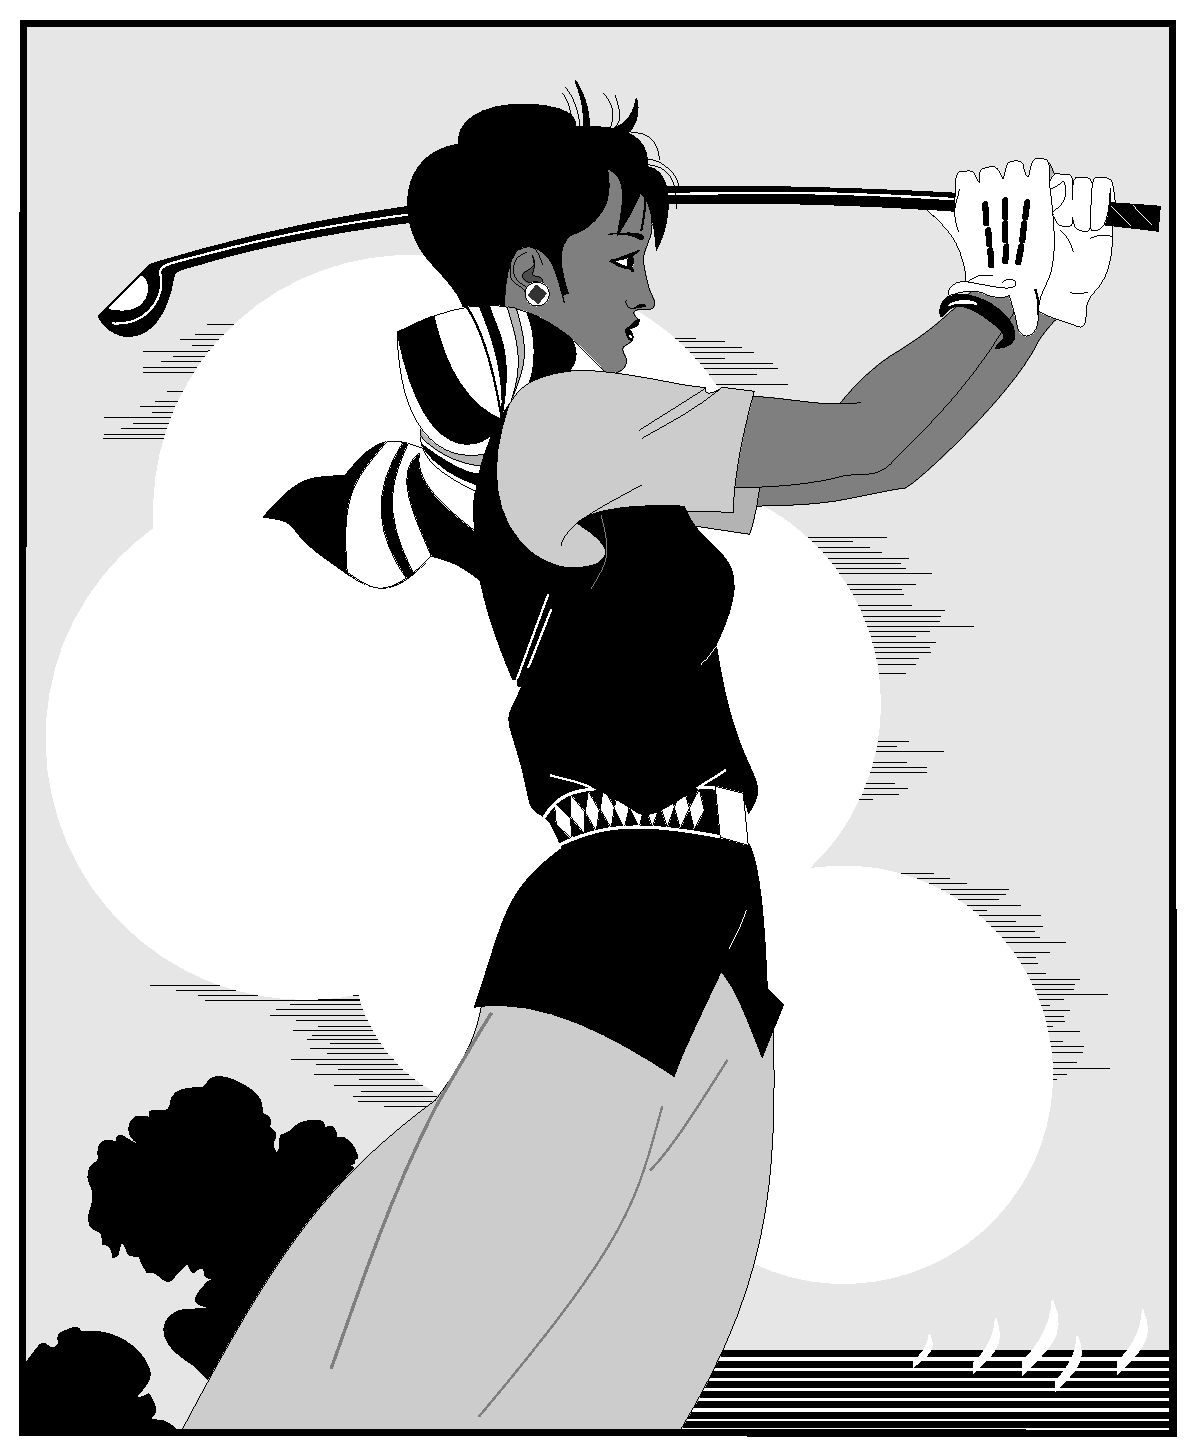
\includegraphics[width = 0.4\textwidth]{golfer}
%\bicaption[golfer5]{}{\xiaosi[0]打高尔夫球的人}{Fig.$\!$}{The person playing golf}\vspace{-1em}
\caption{\xiaosi[0]打高尔夫球的人}
\end{figure}

附录中公式的示例:
\begin{align}
a & = b \times c \\
E & = m c^2
\label{eq}
\end{align}

\chapter{这个星球上最好的免费Linux软件列表}[List of the Best Linux Software in our Planet]
\section{系统}

\href{http://fvwm.org/}{FVWM 自从上世纪诞生以来,此星球最强大的窗口管理器。}
推荐基于FVWM的桌面设计hifvwm:\href{https://github.com/dustincys/hifvwm}{https://github.com/dustincys/hifvwm}。

\subsection{hifvwm的优点}

\begin{enumerate}
	\item 即使打开上百个窗口也不会“蒙圈”。计算机性能越来越强大,窗口任务的管理必须要升级到打怪兽级别。
	\item 自动同步Bing搜索主页的壁纸。每次电脑开机,午夜零点自动更新,用户
		也可以手动更新,从此审美再也不疲劳。
	\item 切换窗口自动聚焦到最上面的窗口。使用键盘快捷键切换窗口时候,减少
		操作过程,自动聚焦到目标窗口。这一特性是虚拟窗口必须的人性化设
		计。
	\item 类似window右下角的功能的最小化窗口来显示桌面的功能此处类似
		win7/win10,实现在一个桌面之内操作多个任务。
	\item 任务栏结合标题栏。采用任务栏和标题栏结合,节省空间。
	\item 同类窗口切换。可以在同类窗口之内类似alt-tab的方式切换。
	\item ……
\end{enumerate}

\section{其他}

\href{https://github.com/goldendict/goldendict}{goldendict 星球最强大的桌面字典。}

\href{https://github.com/yarrick/iodine}{iodine,“HIT-WLAN + 锐捷”时代的福音。}

\href{http://www.aircrack-ng.org/}{aircrack,Wifi“安全性评估”工具。}

\href{https://www.ledger-cli.org/}{ledger,前“金融区块链”时代最好的复式记账系统。}

\href{https://orgmode.org/}{orgmode,最强大的笔记系统,从来没有之一。}

\href{https://www.jianguoyun.com/}{坚果云,国内一款支持WebDav的云盘系统,国内真正的云盘没有之一。}

\href{http://www.mutt.org/}{mutt, ``All mail clients suck. This one just sucks less.''}

\section{vim}
实现中英文每一句一行,以及实现每一句折叠断行的简单正则式,tex源码更加乖乖。
\begin{lstlisting}
vnoremap <leader>fae J:s/[.!?]\zs\s\+/\="\r".matchstr(getline('.'), '^\s*')/g<CR>
vnoremap <leader>fac J:s/[。!?]/\=submatch(0)."\n".matchstr(getline('.'), '^\s*')/g<CR>
vnoremap <leader>fle :!fmt -80 -s<CR>
\end{lstlisting}

%\end{appendix}
%% !Mode:: "TeX:UTF-8" 

\begin{publication}
\noindent\textbf{(一)发表的学术论文}
\begin{publist}
\item	XXX,XXX. Static Oxidation Model of Al-Mg/C Dissipation Thermal Protection Materials[J]. Rare Metal Materials and Engineering, 2010, 39(Suppl. 1): 520-524.(SCI~收录,IDS号为~669JS,IF=0.16)
\item XXX,XXX. 精密超声振动切削单晶铜的计算机仿真研究[J]. 系统仿真学报,2007,19(4):738-741,753.(EI~收录号:20071310514841)
\item XXX,XXX. 局部多孔质气体静压轴向轴承静态特性的数值求解[J]. 摩擦学学报,2007(1):68-72.(EI~收录号:20071510544816)
\item XXX,XXX. 硬脆光学晶体材料超精密切削理论研究综述[J]. 机械工程学报,2003,39(8):15-22.(EI~收录号:2004088028875)
\item XXX,XXX. 基于遗传算法的超精密切削加工表面粗糙度预测模型的参数辨识以及切削参数优化[J]. 机械工程学报,2005,41(11):158-162.(EI~收录号:2006039650087)
\item XXX,XXX. Discrete Sliding Mode Cintrok with Fuzzy Adaptive Reaching Law on 6-PEES Parallel Robot[C]. Intelligent System Design and Applications, Jinan, 2006: 649-652.(EI~收录号:20073210746529)
\end{publist}

\noindent\textbf{(二)申请及已获得的专利(无专利时此项不必列出)}
\begin{publist}
\item XXX,XXX. 一种温热外敷药制备方案:中国,88105607.3[P]. 1989-07-26.
\end{publist}

\noindent\textbf{(三)参与的科研项目及获奖情况}
\begin{publist}
\item	XXX,XXX. XX~气体静压轴承技术研究, XX~省自然科学基金项目.课题编号:XXXX.
\item XXX,XXX. XX~静载下预应力混凝土房屋结构设计统一理论. 黑江省科学技术二等奖, 2007.
\end{publist}
%\vfill
%\hangafter=1\hangindent=2em\noindent
%\setlength{\parindent}{2em}
\end{publication}
    % 所发文章
%\begin{ceindex}
  %如果想要手动加索引,注释掉以下这一样,用wordlist环境
\printsubindex*
\end{ceindex}
    % 索引, 根据自己的情况添加或者不添加,选择自动添加或者手工添加。
%\authorization %授权
%%\authorization[saomiao.pdf] %添加扫描页的命令,与上互斥
%% !Mode:: "TeX:UTF-8"
\begin{acknowledgements}
衷心感谢导师~XXX~教授对本人的精心指导。他的言传身教将使我终生受益。

……

感谢哈工大\LaTeX\ 论文模板\hithesis\ !

\end{acknowledgements}
 %致谢
%% !Mode:: "TeX:UTF-8" 

\begin{resume}
XXXX~年~XX~月~XX~日出生于~XXXX。

XXXX~年~XX~月考入~XX~大学~XX~院(系)XX~专业,XXXX~年~XX~月本科毕业并获得~XX~学学士学位。

XXXX~年~XX~月------XXXX~年~XX~月在~XX~大学~XX~院(系)XX~学科学习并获得~XX~学硕士学位。

XXXX~年~XX~月------XXXX~年~XX~月在~XX~大学~XX~院(系)XX~学科学习并获得~XX~学博士学位。

获奖情况:如获三好学生、优秀团干部、X~奖学金等(不含科研学术获奖)。

工作经历:

\textbf{( 除全日制硕士生以外,其余学生均应增列此项。个人简历一般应包含教育经历和工作经历。)}
\end{resume}
          % 博士学位论文有个人简介

%本科书序为:
%% !Mode:: "TeX:UTF-8" 
\begin{conclusions}

学位论文的结论作为论文正文的最后一章单独排写,但不加章标题序号。

结论应是作者在学位论文研究过程中所取得的创新性成果的概要总结,不能与摘要混为一谈。博士学位论文结论应包括论文的主要结果、创新点、展望三部分,在结论中应概括论文的核心观点,明确、客观地指出本研究内容的创新性成果(含新见解、新观点、方法创新、技术创新、理论创新),并指出今后进一步在本研究方向进行研究工作的展望与设想。对所取得的创新性成果应注意从定性和定量两方面给出科学、准确的评价,分(1)、(2)、(3)…条列出,宜用“提出了”、“建立了”等词叙述。

\end{conclusions}
   % 结论
%\bibliographystyle{hithesis}
%\bibliography{reference}
%\authorization %授权
%%\authorization[saomiao.pdf] %添加扫描页的命令,与上互斥
%% !Mode:: "TeX:UTF-8"
\begin{acknowledgements}
衷心感谢导师~XXX~教授对本人的精心指导。他的言传身教将使我终生受益。

……

感谢哈工大\LaTeX\ 论文模板\hithesis\ !

\end{acknowledgements}
 %致谢
%\begin{appendix}%附录
%\chapter{外文资料原文}
\label{cha:engorg}

\title{The title of the English paper}

\textbf{Abstract:} As one of the most widely used techniques in operations
research, \emph{ mathematical programming} is defined as a means of maximizing a
quantity known as \emph{bjective function}, subject to a set of constraints
represented by equations and inequalities. Some known subtopics of mathematical
programming are linear programming, nonlinear programming, multiobjective
programming, goal programming, dynamic programming, and multilevel
programming$^{[1]}$.

It is impossible to cover in a single chapter every concept of mathematical
programming. This chapter introduces only the basic concepts and techniques of
mathematical programming such that readers gain an understanding of them
throughout the book$^{[2,3]}$.


\section{Single-Objective Programming}
The general form of single-objective programming (SOP) is written
as follows,
\begin{equation}\tag*{(123)} % 如果附录中的公式不想让它出现在公式索引中,那就请
                             % 用 \tag*{xxxx}
\left\{\begin{array}{l}
\max \,\,f(x)\\[0.1 cm]
\mbox{subject to:} \\ [0.1 cm]
\qquad g_j(x)\le 0,\quad j=1,2,\cdots,p
\end{array}\right.
\end{equation}
which maximizes a real-valued function $f$ of
$x=(x_1,x_2,\cdots,x_n)$ subject to a set of constraints.

\newtheorem{mpdef}{Definition}[chapter]
\begin{mpdef}
In SOP, we call $x$ a decision vector, and
$x_1,x_2,\cdots,x_n$ decision variables. The function
$f$ is called the objective function. The set
\begin{equation}\tag*{(456)} % 这里同理,其它不再一一指定。
S=\left\{x\in\Re^n\bigm|g_j(x)\le 0,\,j=1,2,\cdots,p\right\}
\end{equation}
is called the feasible set. An element $x$ in $S$ is called a
feasible solution.
\end{mpdef}

\newtheorem{mpdefop}[mpdef]{Definition}
\begin{mpdefop}
A feasible solution $x^*$ is called the optimal
solution of SOP if and only if
\begin{equation}
f(x^*)\ge f(x)
\end{equation}
for any feasible solution $x$.
\end{mpdefop}

One of the outstanding contributions to mathematical programming was known as
the Kuhn-Tucker conditions\ref{eq:ktc}. In order to introduce them, let us give
some definitions. An inequality constraint $g_j(x)\le 0$ is said to be active at
a point $x^*$ if $g_j(x^*)=0$. A point $x^*$ satisfying $g_j(x^*)\le 0$ is said
to be regular if the gradient vectors $\nabla g_j(x)$ of all active constraints
are linearly independent.

Let $x^*$ be a regular point of the constraints of SOP and assume that all the
functions $f(x)$ and $g_j(x),j=1,2,\cdots,p$ are differentiable. If $x^*$ is a
local optimal solution, then there exist Lagrange multipliers
$\lambda_j,j=1,2,\cdots,p$ such that the following Kuhn-Tucker conditions hold,
\begin{equation}
\label{eq:ktc}
\left\{\begin{array}{l}
    \nabla f(x^*)-\sum\limits_{j=1}^p\lambda_j\nabla g_j(x^*)=0\\[0.3cm]
    \lambda_jg_j(x^*)=0,\quad j=1,2,\cdots,p\\[0.2cm]
    \lambda_j\ge 0,\quad j=1,2,\cdots,p.
\end{array}\right.
\end{equation}
If all the functions $f(x)$ and $g_j(x),j=1,2,\cdots,p$ are convex and
differentiable, and the point $x^*$ satisfies the Kuhn-Tucker conditions
(\ref{eq:ktc}), then it has been proved that the point $x^*$ is a global optimal
solution of SOP.

\subsection{Linear Programming}
\label{sec:lp}

If the functions $f(x),g_j(x),j=1,2,\cdots,p$ are all linear, then SOP is called
a {\em linear programming}.

The feasible set of linear is always convex. A point $x$ is called an extreme
point of convex set $S$ if $x\in S$ and $x$ cannot be expressed as a convex
combination of two points in $S$. It has been shown that the optimal solution to
linear programming corresponds to an extreme point of its feasible set provided
that the feasible set $S$ is bounded. This fact is the basis of the {\em simplex
  algorithm} which was developed by Dantzig as a very efficient method for
solving linear programming.
\begin{table}[ht]
\centering
  \centering
  \caption*{Table~1\hskip1em This is an example for manually numbered table, which
    would not appear in the list of tables}
  \label{tab:badtabular2}
  \begin{tabular}[c]{|m{1.5cm}|c|c|c|c|c|c|}\hline
    \multicolumn{2}{|c|}{Network Topology} & \# of nodes &
    \multicolumn{3}{c|}{\# of clients} & Server \\\hline
    GT-ITM & Waxman Transit-Stub & 600 &
    \multirow{2}{2em}{2\%}&
    \multirow{2}{2em}{10\%}&
    \multirow{2}{2em}{50\%}&
    \multirow{2}{1.2in}{Max. Connectivity}\\\cline{1-3}
    \multicolumn{2}{|c|}{Inet-2.1} & 6000 & & & &\\\hline
    & \multicolumn{2}{c|}{ABCDEF} &\multicolumn{4}{c|}{} \\\hline
\end{tabular}
\end{table}

Roughly speaking, the simplex algorithm examines only the extreme points of the
feasible set, rather than all feasible points. At first, the simplex algorithm
selects an extreme point as the initial point. The successive extreme point is
selected so as to improve the objective function value. The procedure is
repeated until no improvement in objective function value can be made. The last
extreme point is the optimal solution.

\subsection{Nonlinear Programming}

If at least one of the functions $f(x),g_j(x),j=1,2,\cdots,p$ is nonlinear, then
SOP is called a {\em nonlinear programming}.

A large number of classical optimization methods have been developed to treat
special-structural nonlinear programming based on the mathematical theory
concerned with analyzing the structure of problems.

Now we consider a nonlinear programming which is confronted solely with
maximizing a real-valued function with domain $\Re^n$.  Whether derivatives are
available or not, the usual strategy is first to select a point in $\Re^n$ which
is thought to be the most likely place where the maximum exists. If there is no
information available on which to base such a selection, a point is chosen at
random. From this first point an attempt is made to construct a sequence of
points, each of which yields an improved objective function value over its
predecessor. The next point to be added to the sequence is chosen by analyzing
the behavior of the function at the previous points. This construction continues
until some termination criterion is met. Methods based upon this strategy are
called {\em ascent methods}, which can be classified as {\em direct methods},
{\em gradient methods}, and {\em Hessian methods} according to the information
about the behavior of objective function $f$. Direct methods require only that
the function can be evaluated at each point. Gradient methods require the
evaluation of first derivatives of $f$. Hessian methods require the evaluation
of second derivatives. In fact, there is no superior method for all
problems. The efficiency of a method is very much dependent upon the objective
function.

\subsection{Integer Programming}

{\em Integer programming} is a special mathematical programming in which all of
the variables are assumed to be only integer values. When there are not only
integer variables but also conventional continuous variables, we call it {\em
  mixed integer programming}. If all the variables are assumed either 0 or 1,
then the problem is termed a {\em zero-one programming}. Although integer
programming can be solved by an {\em exhaustive enumeration} theoretically, it
is impractical to solve realistically sized integer programming problems. The
most successful algorithm so far found to solve integer programming is called
the {\em branch-and-bound enumeration} developed by Balas (1965) and Dakin
(1965). The other technique to integer programming is the {\em cutting plane
  method} developed by Gomory (1959).

\hfill\textit{Uncertain Programming\/}\quad(\textsl{BaoDing Liu, 2006.2})

\section*{References}
\noindent{\itshape NOTE: These references are only for demonstration. They are
  not real citations in the original text.}

\begin{translationbib}
\item Donald E. Knuth. The \TeX book. Addison-Wesley, 1984. ISBN: 0-201-13448-9
\item Paul W. Abrahams, Karl Berry and Kathryn A. Hargreaves. \TeX\ for the
  Impatient. Addison-Wesley, 1990. ISBN: 0-201-51375-7
\item David Salomon. The advanced \TeX book.  New York : Springer, 1995. ISBN:0-387-94556-3
\end{translationbib}

\chapter{外文资料的调研阅读报告或书面翻译}

\title{英文资料的中文标题}

{\heiti 摘要:} 本章为外文资料翻译内容。如果有摘要可以直接写上来,这部分好像没有
明确的规定。

\section{单目标规划}
北冥有鱼,其名为鲲。鲲之大,不知其几千里也。化而为鸟,其名为鹏。鹏之背,不知其几
千里也。怒而飞,其翼若垂天之云。是鸟也,海运则将徙于南冥。南冥者,天池也。
\begin{equation}\tag*{(123)}
 p(y|\mathbf{x}) = \frac{p(\mathbf{x},y)}{p(\mathbf{x})}=
\frac{p(\mathbf{x}|y)p(y)}{p(\mathbf{x})}
\end{equation}

吾生也有涯,而知也无涯。以有涯随无涯,殆已!已而为知者,殆而已矣!为善无近名,为
恶无近刑,缘督以为经,可以保身,可以全生,可以养亲,可以尽年。

\subsection{线性规划}
庖丁为文惠君解牛,手之所触,肩之所倚,足之所履,膝之所倚,砉然响然,奏刀騞然,莫
不中音,合于桑林之舞,乃中经首之会。
\begin{table}[ht]
\centering
  \centering
  \caption*{表~1\hskip1em 这是手动编号但不出现在索引中的一个表格例子}
  \label{tab:badtabular3}
  \begin{tabular}[c]{|m{1.5cm}|c|c|c|c|c|c|}\hline
    \multicolumn{2}{|c|}{Network Topology} & \# of nodes &
    \multicolumn{3}{c|}{\# of clients} & Server \\\hline
    GT-ITM & Waxman Transit-Stub & 600 &
    \multirow{2}{2em}{2\%}&
    \multirow{2}{2em}{10\%}&
    \multirow{2}{2em}{50\%}&
    \multirow{2}{1.2in}{Max. Connectivity}\\\cline{1-3}
    \multicolumn{2}{|c|}{Inet-2.1} & 6000 & & & &\\\hline
    & \multicolumn{2}{c|}{ABCDEF} &\multicolumn{4}{c|}{} \\\hline
\end{tabular}
\end{table}

文惠君曰:“嘻,善哉!技盖至此乎?”庖丁释刀对曰:“臣之所好者道也,进乎技矣。始臣之
解牛之时,所见无非全牛者;三年之后,未尝见全牛也;方今之时,臣以神遇而不以目视,
官知止而神欲行。依乎天理,批大郤,导大窾,因其固然。技经肯綮之未尝,而况大坬乎!
良庖岁更刀,割也;族庖月更刀,折也;今臣之刀十九年矣,所解数千牛矣,而刀刃若新发
于硎。彼节者有间而刀刃者无厚,以无厚入有间,恢恢乎其于游刃必有余地矣。是以十九年
而刀刃若新发于硎。虽然,每至于族,吾见其难为,怵然为戒,视为止,行为迟,动刀甚微,
謋然已解,如土委地。提刀而立,为之而四顾,为之踌躇满志,善刀而藏之。”

文惠君曰:“善哉!吾闻庖丁之言,得养生焉。”


\subsection{非线性规划}
孔子与柳下季为友,柳下季之弟名曰盗跖。盗跖从卒九千人,横行天下,侵暴诸侯。穴室枢
户,驱人牛马,取人妇女。贪得忘亲,不顾父母兄弟,不祭先祖。所过之邑,大国守城,小
国入保,万民苦之。孔子谓柳下季曰:“夫为人父者,必能诏其子;为人兄者,必能教其弟。
若父不能诏其子,兄不能教其弟,则无贵父子兄弟之亲矣。今先生,世之才士也,弟为盗
跖,为天下害,而弗能教也,丘窃为先生羞之。丘请为先生往说之。”

柳下季曰:“先生言为人父者必能诏其子,为人兄者必能教其弟,若子不听父之诏,弟不受
兄之教,虽今先生之辩,将奈之何哉?且跖之为人也,心如涌泉,意如飘风,强足以距敌,
辩足以饰非。顺其心则喜,逆其心则怒,易辱人以言。先生必无往。”

孔子不听,颜回为驭,子贡为右,往见盗跖。

\subsection{整数规划}
盗跖乃方休卒徒大山之阳,脍人肝而餔之。孔子下车而前,见谒者曰:“鲁人孔丘,闻将军
高义,敬再拜谒者。”谒者入通。盗跖闻之大怒,目如明星,发上指冠,曰:“此夫鲁国之
巧伪人孔丘非邪?为我告之:尔作言造语,妄称文、武,冠枝木之冠,带死牛之胁,多辞缪
说,不耕而食,不织而衣,摇唇鼓舌,擅生是非,以迷天下之主,使天下学士不反其本,妄
作孝弟,而侥幸于封侯富贵者也。子之罪大极重,疾走归!不然,我将以子肝益昼餔之膳。”


\chapter{其它附录}
前面两个附录主要是给本科生做例子。其它附录的内容可以放到这里,当然如果你愿意,可
以把这部分也放到独立的文件中,然后将其到主文件中。
%本科生翻译论文
%\end{appendix}

%开题/中期书序:


\end{document}
